% !TEX root = Projektdokumentation.tex
\section{Anhang}

%\subsection{Detaillierte Zeitplanung}
%\label{app:Zeitplanung}
%\tabelleAnhang{ZeitplanungKomplett}

%\subsection{Gantt-Diagramm}
%\label{app:Gantt}
%\begin{sideways}
%\begin{ganttchart}[
hgrid,
vgrid,
x unit=4mm,
time slot format=isodate
]{2016-04-12}{2016-05-31}
\gantttitlecalendar{year, month, day, week=3, weekday} \\

\ganttbar{}{2016-04-14}{2016-04-17}

\end{ganttchart}

%\end{sideways}


\subsection{API Call: Register as a new user}
\label{app:API_register}
\tabelleAnhang{WebService/register}

\subsection{API Call: Login}
\label{app:API_login}
\tabelleAnhang{WebService/login}

\subsection{API Call: Register a new room}
\label{app:API_register_room}
\tabelleAnhang{WebService/newRoom}

\subsection{API Call: Delete a room}
\label{app:API_delete_room}
\tabelleAnhang{WebService/deleteRoom}

\subsection{API Call: Show a specific room}
\label{app:API_show_room}
\tabelleAnhang{WebService/getRoom}

\subsection{API Call: Show all rooms}
\label{app:API_show_rooms}
\tabelleAnhang{WebService/getRooms}

\subsection{API Call: Register a new device}
\label{app:API_register_device}
\tabelleAnhang{WebService/registerDevice}

\subsection{API Call: Show a specific device}
\label{app:API_get_device}
\tabelleAnhang{WebService/getDevice}

\subsection{API Call: Delete a specific device}
\label{app:API_delete_device}
\tabelleAnhang{WebService/deleteDevice}

\subsection{API Call: Show all devices}
\label{app:API_show_devices}
\tabelleAnhang{WebService/getDevices}

\subsection{API Call: Send a command to a specific device}
\label{app:API_dend_command}
\tabelleAnhang{WebService/doCommand}




%\subsection{Projektdokumentation Sommersemester 2015}
%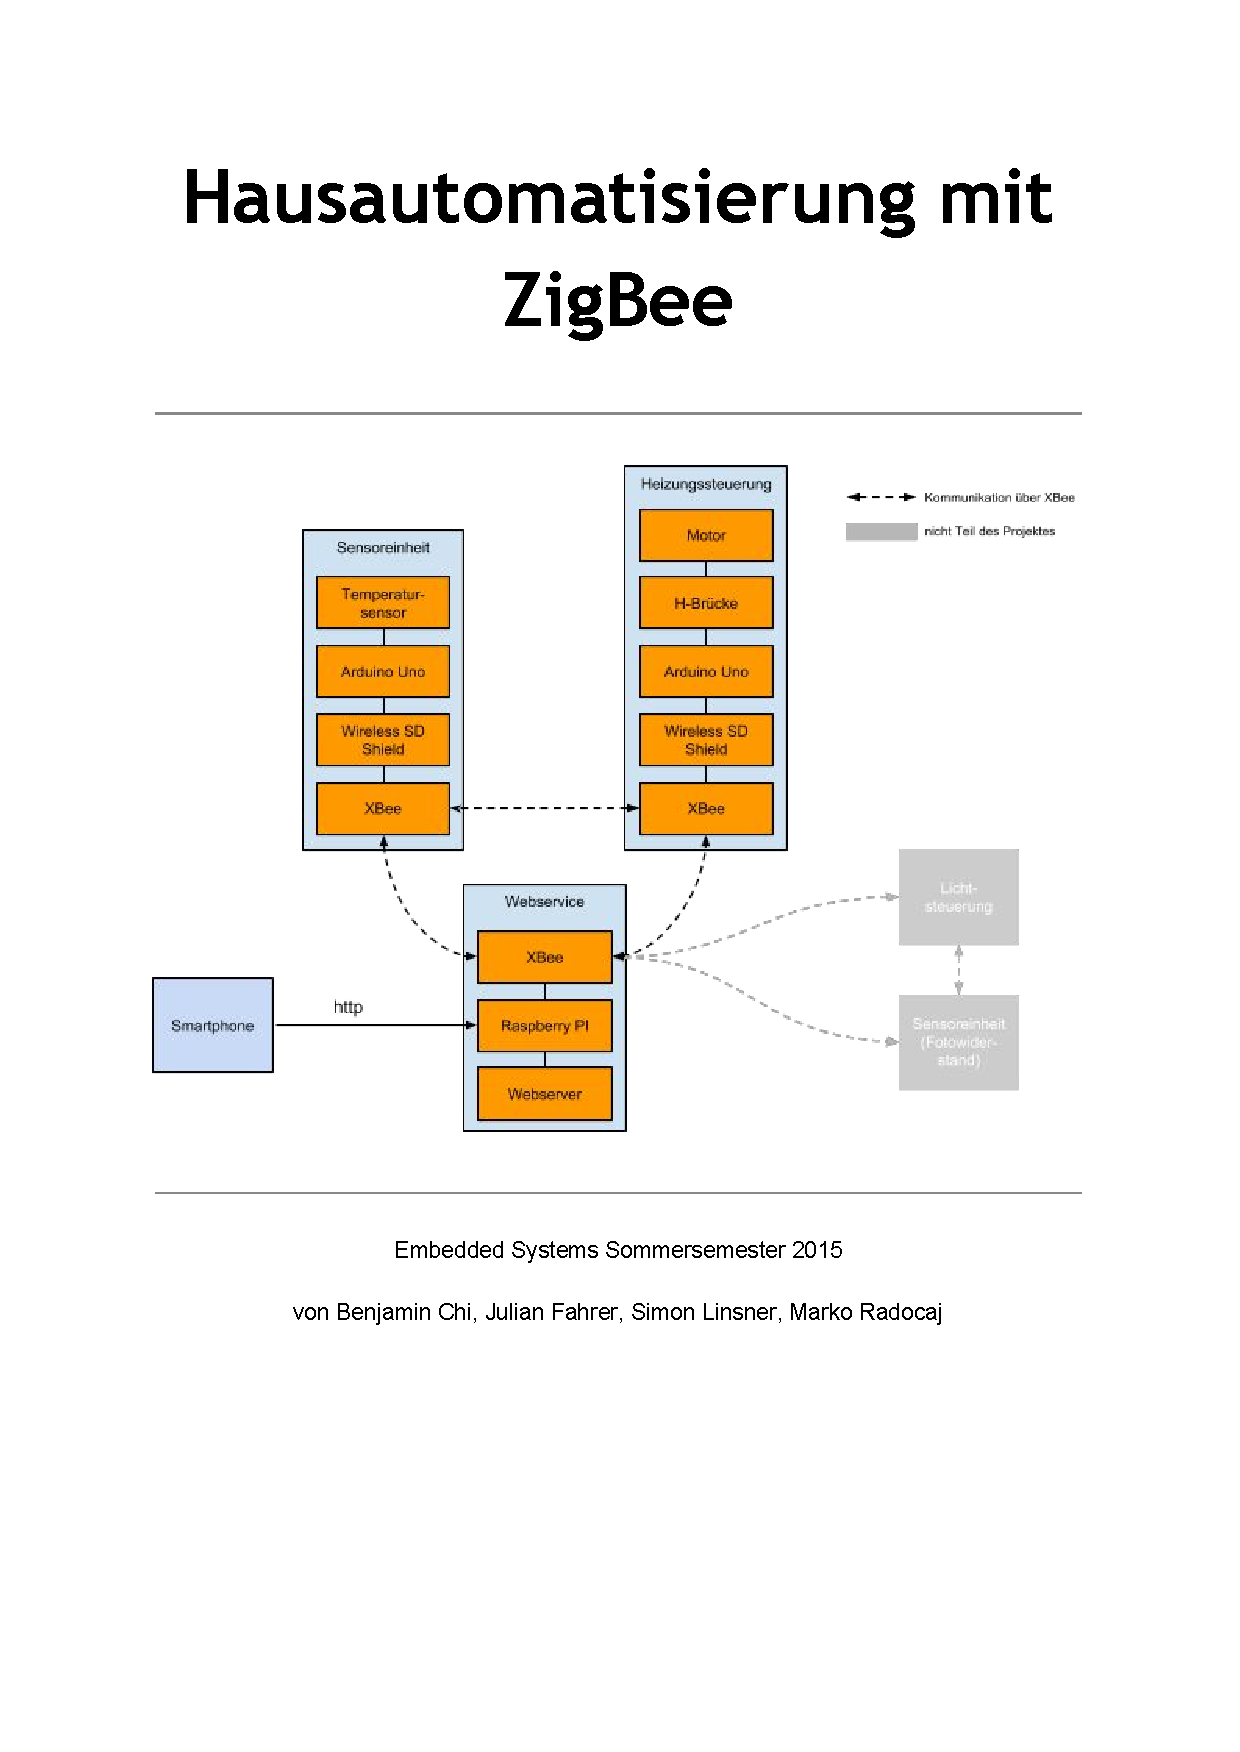
\includepdf[pagecommand={\thispagestyle{headings}},
%  pages=1-23, scale=0.8, frame=true]{Anhang/Dokumentation_SoSe2015.pdf}

